\documentclass[12pt,a4paper,twoside]{report}
% -------------------------------------------------------------------- %
% Pacotes

\usepackage[utf8]{inputenc}
\usepackage[T1]{fontenc}
\usepackage[brazil]{babel}
\usepackage[fixlanguage]{babelbib}
\usepackage[pdftex]{graphicx}      % usamos arquivos pdf/png como figuras
\usepackage{setspace}              % espaçamento flexvel
\usepackage{indentfirst}           % indentação do primeiro parágrafo
\usepackage{makeidx}               % índice remissivo
\usepackage[nottoc]{tocbibind}     % acrescentamos a bibliografia/indice/conteudo no Table of Contents
\usepackage{courier}               % usa o Adobe Courier no lugar de Computer Modern Typewriter
\usepackage{type1cm}               % fontes realmente escaláveis
\usepackage{titletoc}
\usepackage{ucs}
\usepackage[font=small,format=plain,labelfont=bf,up,textfont=it,up]{caption}
\usepackage[usenames,svgnames,dvipsnames]{xcolor}
\usepackage[a4paper,top=2.54cm,bottom=2.0cm,left=2.0cm,right=2.54cm]{geometry} % margens
\usepackage{amsmath}

\usepackage[pdftex,plainpages=false,pdfpagelabels,pagebackref,colorlinks=true,citecolor=DarkGreen,
linkcolor=NavyBlue,urlcolor=DarkRed,filecolor=green,bookmarksopen=true]{hyperref} % links coloridos
\usepackage[all]{hypcap}                % soluciona o problema com o hyperref e capítulos
\usepackage[square,sort,nonamebreak,comma]{natbib}  % citação bibliográfica alpha
\fontsize{60}{62}\usefont{OT1}{cmr}{m}{n}{\selectfont}
\usepackage{upquote}                    % formata apóstrofes '
\usepackage{textcomp}

% Para formatar corretamente as URLs
\usepackage{url}
% -------------------------------------------------------------------- %
% Cabeçalhos similares ao TAOCP de Donald E. Knuth
\usepackage{fancyhdr}
\pagestyle{fancy}
\fancyhf{}
\renewcommand{\chaptermark}[1]{\markboth{\MakeUppercase{#1}}{}}
\renewcommand{\sectionmark}[1]{\markright{\MakeUppercase{#1}}{}}
\renewcommand{\headrulewidth}{0pt}

% -------------------------------------------------------------------- %
\graphicspath{{./imagens/}}        % caminho das figuras
\frenchspacing                     % arruma o espaço: id est (i.e.) e exempli gratia (e.g.)
\urlstyle{same}                    % URL com o mesmo estilo do texto e no mono-spaced
\makeindex                         % para o índice remissivo
\raggedbottom                      % para no permitir espaços extras no texto
\fontsize{60}{62}\usefont{OT1}{cmr}{m}{n}{\selectfont}
\cleardoublepage
\normalsize

% -------------------------------------------------------------------- %
% Cores para formatação de código
\usepackage{color}
\definecolor{vermelho}{rgb}{0.6,0,0} % para strings
\definecolor{verde}{rgb}{0.25,0.5,0.35} % para comentários
\definecolor{roxo}{rgb}{0.5,0,0.35} % para palavras-chaves
\definecolor{azul}{rgb}{0.25,0.35,0.75} % para strings
\definecolor{cinza-claro}{gray}{0.95}
% -------------------------------------------------------------------- %
% Opções de listagem usados para o código fonte
% Ref: http://en.wikibooks.org/wiki/LaTeX/Packages/Listings



\usepackage{listings}           % para formatar código-fonte (ex. em Java)


\lstset{ %
language=[Objective]Caml,  % seleciona a linguagem do código (aqui em lstlang0.sty
basicstyle=\footnotesize\ttfamily, % o tamanho da fonte usado no código
commentstyle=\color{verde}\bfseries,  % formatação de comentários
stringstyle=\color{azul},    % formatação de strings
upquote=true,
numbers=left,                   % onde colocar os números de linha
numberstyle=\tiny,  % o tamanho da fonte usada para a numeração das linhas
stepnumber=1,                   % o intervalo entre dois números de linhas. Se for 1, numera cada uma.
numbersep=5pt,                  % how far the line-numbers are from the code
showspaces=false,               % show spaces adding particular underscores
showstringspaces=false,         % underline spaces within strings
showtabs=false,                 % show tabs within strings adding particular underscores
keywordstyle=\color{roxo}\bfseries,
keywordstyle=[1]\color{roxo}\bfseries,
keywordstyle=[2]\color{verde}\bfseries,
%        keywordstyle=[3]\textbf,    %
%        keywordstyle=[4]\textbf,   \sqrt{\sqrt{}} %
frame=b,                   % adds a frame around the code
framerule=0.6pt,
tabsize=2,                      % sets default tabsize to 2 spaces
captionpos=t,                   % sets the caption-position to top
breaklines=true,                % sets automatic line breaking
breakatwhitespace=false,        % sets if automatic breaks should only happen at whitespace
escapeinside={\%*}{*)},         % if you want to add a comment within your code
backgroundcolor=\color[rgb]{1.0,1.0,1.0}, % choose the background color.
rulecolor=\color[rgb]{0.8,0.8,0.8},
extendedchars=true,
xleftmargin=10pt,
xrightmargin=10pt,
framexleftmargin=10pt,
framexrightmargin=10pt,
literate={â}{{\^{a}}}1  % para formatar corretamente os acentos do Português ao usar utf8
    {ê}{{\^{e}}}1
    {ô}{{\^{o}}}1
    {Â}{{\^{A}}}1
    {Ê}{{\^{E}}}1
    {Ô}{{\^{O}}}1
    {á}{{\'{a}}}1
    {é}{{\'{e}}}1
    {í}{{\'{i}}}1
    {ó}{{\'{o}}}1
    {ú}{{\'{u}}}1
    {Á}{{\'{A}}}1
    {É}{{\'{E}}}1
    {Í}{{\'{I}}}1
    {Ó}{{\'{O}}}1
    {Ú}{{\'{U}}}1
    {à}{{\`{a}}}1
    {À}{{\`{A}}}1
    {ã}{{\~{a}}}1
    {õ}{{\~{o}}}1
    {Ã}{{\~{A}}}1
    {Õ}{{\~{O}}}1
    {ç}{{\c{c}}}1
    {Ç}{{\c{C}}}1
    {ü}{{\"u}}1
    {Ü}{{\"U}}1
}

\renewcommand{\lstlistingname}{Listagem}
\renewcommand{\lstlistlistingname}{Lista de Listagens}

% Definição de novos estilos
\lstdefinestyle{Bash}
    {language=bash,frame=single,numbers=none,basicstyle=\footnotesize\ttfamily,
     morekeywords={cp,mkdir,sudo,tar}}

% Definição de novos ambientes
\lstnewenvironment{terminal}
  {\lstset{style=Bash}}
  {}

\lstnewenvironment{ocaml}
  {\lstset{basicstyle=\scriptsize\ttfamily,
           frame=single,
           frameround=tttt,
           framerule=2pt,
           numbers=none,
           rulecolor=\color{Salmon}}}
  {}

\lstnewenvironment{xml}
   {\lstset{language=XML,frame=single,numbers=none}}
   {}

\lstnewenvironment{interprete}
  {\lstset{frame=single,
            frameround=tttt,
            numbers=none,
            basicstyle=\ttfamily,
            framerule=2pt,
            rulecolor=\color{CadetBlue}}}
  {}
% Formata o caption da listagem
% \DeclareCaptionFont{blue}{\color{blue}}

% \captionsetup[lstlisting]{singlelinecheck=false, labelfont={blue}, textfont={blue}}
\usepackage{caption}
\DeclareCaptionFont{white}{\color{white}}
\DeclareCaptionFormat{listing}{\colorbox[cmyk]{0.43, 0.35, 0.35,0.01}{\parbox{\textwidth}{\hspace{15pt}#1#2#3}}}
\captionsetup[lstlisting]{format=listing,labelfont=white,textfont=white, singlelinecheck=false, margin=0pt, font={bf,footnotesize}}

\newcommand{\ListingsPath}{./codigos}
% Inclui o nome do arquivo como Caption
\newcommand{\filelisting}[2][]{%
    \lstinputlisting[caption={\texttt{\detokenize{#2}}},#1]{\ListingsPath/#2}%
}

% ---------------------------------------------------------------------------- %

% ---------------------------------------------------------------------------- %

\title{Construção de um compilador de Lua para Parrot Virtual Machine usando Objective Caml}
\date{}
\author{Guilherme Pacheco de Oliveira \\
\texttt{\small \url{guilherme.061@gmail.com}}
\vspace{1cm} \\
Faculdade de Computação \\
Universidade Federal de Uberlândia
}
\date{\today}

%\includeonly{cap-clojure,magical,short}
\begin{document}
  \maketitle
% -------------------------------------------------------------------- %
% Listas de figuras, tabelas e códigos criadas automaticamente
\listoffigures
\listoftables
\lstlistoflistings
% -------------------------------------------------------------------- %

% -------------------------------------------------------------------- %
% Sumário
\tableofcontents

% Capítulos do trabalho

% cabeçalho para as páginas de todos os capítulos
\fancyhead[RE,LO]{\thesection}

%\singlespacing              % espaçamento simples
\setlength{\parskip}{0.15in} % espaçamento entre paragráfos

\chapter{Introdução}
Este documento foi escrito para documentar o processo de instalação de
todas as ferramentas necessárias para a construção de um compilador da
Linguagem Lua para a máquina virtual Parrot, utilizando a linguagem
Ocaml para fazer a implementação.

Um segundo objetivo é mostrar uma série de programas simples na
linguagem Lua e sua versão na linguagem PASM, que é a linguagem
assembly utilizada pela Parrot, afim de estabelecer um guia sobre a
saída dos programas que passarão pelo compilador.

Outro objetivo é adquirir conhecimento sobre a linguagem Lua, ter um
contato inicial com OCaml e conhecer como funciona a máquina virtual
Parrot, suas linguagens de Assembly e bytecode e de compiladores já
existentes

O Sistema Operacional utilizado é OS X El Capitain 10.11.6

\chapter{Instalação dos componentes}
\section{Homebrew}
Homebrew é um gerenciador de pacotes para Mac OS X, escrito em Ruby, e
é responsável por instalar pacotes nos diretórios adequados e fazer
adequadamente a configuração desses pacotes, instalá-lo facilita todo
o processo de instalação dos componentes necessários.

Para instalar o homebrew basta digitar no terminal:

\begin{terminal}
$ /usr/bin/ruby -e "\$(curl -fsSL https://raw.githubusercontent.com/Homebrew/install/master/install)"
\end{terminal}


\section{Lua}
\subsection{Instalação e Teste}
Para instalar Lua através do homebrew, basta digitar no terminal:
\begin{terminal}
$ brew install lua
\end{terminal}
Resultado:
\begin{figure}[!ht]
\centering
\caption{Instalando e testando LUA}
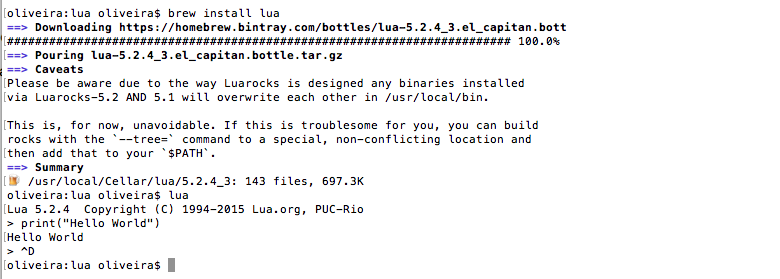
\includegraphics[scale=0.27]{imagens/brew-lua.png}
\end{figure}
\subsection{Informações sobre a linguagem Lua}
A principal referência para Lua é a documentação em seu site oficial [1].
Lua é uma linguagem de programação de extensão, projetada para dar suporte à outras linguagens de programação procedimental e planejada para ser usada como uma linguagem de script leve e facilmente embarcável, é implementada em C.



\section{Ocaml}
\subsection{Instalação e Teste}
Novamente através do homebrew, basta digitar:
\begin{terminal}
$ brew install ocaml
\end{terminal}
Resultado:
\begin{figure}[!ht]
\centering
\caption{Instalando e testando OCaml}
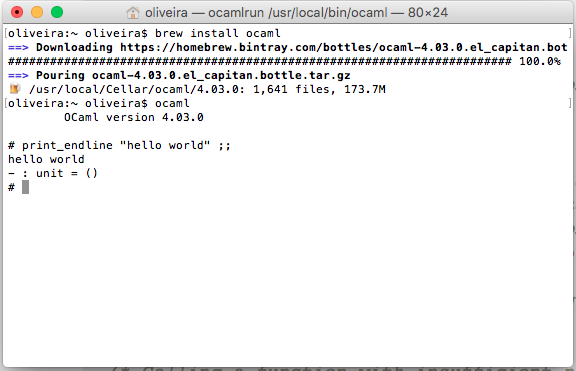
\includegraphics[scale=0.27]{imagens/brew-ocaml.png}
\end{figure}
\subsection{Informações sobre a linguagem OCaml}
A documentação oficial do OCaml [2] possui manuais, licenças, documentos e algumas dicas sobre como programar adequadamente na linguagem.
OCaml é uma linguagem de programação funcional, imperativa e orientada à objetos.

\section{Parrot Virtual Machine}

\subsection{Instalação e Teste}
Digitar no Terminal:
\begin{terminal}
$ brew install parrot
\end{terminal}
Resultado:
\begin{figure}[!ht]
\centering
\caption{Instalando e testando Parrot}
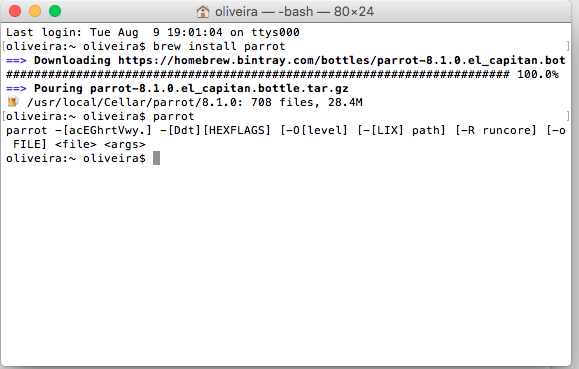
\includegraphics[scale=0.27]{imagens/brew-parrot.png}
\end{figure}
\subsection{Informações sobre a Parrot Virtual Machine}
A máquina virtual Parrot é utilizada principalmente para linguagens dinâmicas como Perl, Python, Ruby e PHP, seu design
foi originalmente feito para trabalhar com a versão 6 de Perl, mas seu uso foi expandido como uma maquina virtual dinâmica
e de proposito geral, apta a lidar com qualquer linguagem de programação de alto nível. [3]

Parrot pode ser programada em diversas linguagens, os dois mais utilizados são:
Parrot Assembly Language (PASM): É a linguagem de mais baixo nível utilizada pela Parrot, muito similar a um assembly tradicional.
Parrot Intermediate Representation(PIR): De mais alto nível que PASM, também um pouco mais facil de se utilizar e mais utilizada.

Fazendo alguns testes com PASM e PIR:
\lstinputlisting[caption={Output Simples em Parrot Assembly Language}]{codigos/parrot/news.pasm}
Para executar o código:
\begin{terminal}
$ parrot news.pasm
\end{terminal}

\lstinputlisting[caption={Output Simples em Parrot Intermediate Representation}]{codigos/parrot/hello.pir}
Para executar o código:
\begin{terminal}
$ parrot hello.pir
\end{terminal}

Os arquivos PASM e PIR são convertidos para Parrot Bytecode (PBC) e somente então são executados pela máquina virutal, é possível obter o arquivo .pbc através comando:
\begin{terminal}
$ parrot -o output.pbc input.pasm
\end{terminal}

De acordo com a documentação oficial, o Compilador Intermediário de Parrot é capaz de traduzir códigos PIR para PASM através do comando:
\begin{terminal}
$ parrot -o output.pasm input.pir
\end{terminal}
Mas essa execução resultou em um código bytecode invés do assembly.

Apesar da documentação oficial enfatizar que PIR é mais utilizado e mais recomendado para o desenvolvimento de compiladores para Parrot, o alvo será a linguagem Assembly PASM.

\subsection{Parrot Assembly Language (PASM)}
A linguagem PASM é muito similar a um assembly tradicional, com exceção do fato de que algumas instruções permitem o acesso a algumas funções dinâmicas de alto nível do sistema Parrot.

Parrot é uma maquina virtual baseada em registradores, há um número ilimitado de registradores que não precisam ser instanciados antes de serem utilizados, a maquina virtual se certifica de criar os registradores de acordo com a sua necessidade,
tal como fazer a reutilização e se livrar de registradores que não estão mais sendo utilizados, todos os registradores começam com o símbolo "\$" e existem 4 tipos de dados, cada um com suas regras:


Strings: Registradores de strings começam com um S, por exemplo: "\$S10" \\
Inteiros: Registradores de inteiros começam com um I, por exemplo: "\$I10" \\
Número: Registradores de números de ponto flutuante, começam com a letra N, por exemplo: "\$N10" \\
PMC: São tipos de dados utilizados em orientação a objetos, podem ser utilizados para guardar vários tipos de dados, começam com a letra P, por exemplo: "\$P10" \\
\\
Para mais referêcias sobre PASM, consultar [4], [7] para os opcodes e [8] para exemplos.

\subsection{Parrot Intermediate Representation (PIR)}
A maior dos compiladores possuem como alvo o PIR, inclusive o que será
utilizado para estudar qual o comportamento um compilador deve ter ao
gerar o assembly.
A própria máquina virtual Parrot possui um módulo intermediário capaz
de interpretar a linguagem PIR e gerar o bytecode ou o próprio
assembly (PASM), além disso, existem compiladores capaz de realizar a
mesma tarefa.

PIR é de nível mais alto que assembly mas ainda muito próximo do nível
de máquina, o principal benefício é a facilidade em programar em PIR
em comparação com a programação em PASM, além disso, ela foi feita
para compiladores de linguagens de alto nível gerarem código PIR para
trabalhar com a maquina Parrot.
Mais informações sobre PIR e sua sintaxe podem ser encontradas em [5].

\chapter{Compilação de Código Ruby para Parrot Intermediate Representation (PIR)}
O compilador que será utilizado será o Cardinal [6], é um compilador
da linguagem Ruby para a máquina virtual Parrot capaz de gerar código
o código intermediário (PIR) como saída.

A documentação do compilador é simples e clara, para baixar o
compilador basta digitar no terminal:
\begin{terminal}
$ git clone git://github.com/parrot/cardinal.git
\end{terminal}
Entre as várias opções de instalação, é possível faze-la utilizando do
próprio parrot, para isso basta entrar na pasta onde foi baixado o
Cardinal e digitar:
\begin{terminal}
$ winxed setup.winxed build
\end{terminal}

Para compilar é necessário estar na pasta de instalação e o comando é:
\begin{terminal}
$ parrot cardinal.pbc [arquivo].rb
\end{terminal}
Sendo o arquivo o diretório do arquivo Ruby que se deseja executar,
para gerar o PIR o comando é:
\begin{terminal}
$ parrot cardinal.pbc -o [output].pir --target=pir [arquivo].rb
\end{terminal}
Sendo output o diretório onde será salvo o arquivo PIR.

\subsubsection{Exemplo}
\lstinputlisting[caption={Programa nano 01 em Ruby}]{codigos/ruby/nano01.rb}
Compilação do Código Ruby:
\begin{terminal}
$ parrot /Users/oliveira/cardinal/cardinal/cardinal.pbc -o
../parrot/nano01.pir --target=pir nano01.rb
\end{terminal}
\lstinputlisting[caption={Programa nano 01 em PIR}]{codigos/parrot/pir/nano01.pir}

A compilação dos programas Ruby não foi bem sucedida para todos os programas, além disso, programas que utilizavam a linha de código a seguir, que é utilizada para pegar dados do usuário, compilavam mas não funcionavam na máquina virtual.
\begin{terminal}
input = gets.chomp
\end{terminal}


\chapter{Códigos LUA e Parrot Assembly (PASM)}

Os códigos PASM dessa seção foram feitos manualmente, não foram utilizados compiladores para esse fim.

\subsection{Nano Programas}
\subsubsection{Nano 01}
\lstinputlisting[caption={Programa nano 01 em Lua}]{codigos/lua/nano01.lua}
\lstinputlisting[caption={Programa nano 01 em PASM}]{codigos/parrot/pasm/nano01.pasm}

\subsubsection{Nano 02}
\lstinputlisting[caption={Programa nano 02 em Lua}]{codigos/lua/nano02.lua}
\lstinputlisting[caption={Programa nano 02 em PASM}]{codigos/parrot/pasm/nano02.pasm}

\subsubsection{Nano 03}
\lstinputlisting[caption={Programa nano 03 em Lua}]{codigos/lua/nano03.lua}
\lstinputlisting[caption={Programa nano 03 em PASM}]{codigos/parrot/pasm/nano03.pasm}

\subsubsection{Nano 04}
\lstinputlisting[caption={Programa nano 04 em Lua}]{codigos/lua/nano04.lua}
\lstinputlisting[caption={Programa nano 04 em PASM}]{codigos/parrot/pasm/nano04.pasm}

\subsubsection{Nano 05}
\lstinputlisting[caption={Programa nano 05 em Lua}]{codigos/lua/nano05.lua}
\lstinputlisting[caption={Programa nano 05 em PASM}]{codigos/parrot/pasm/nano05.pasm}
Saída:
\begin{terminal}
2
\end{terminal}

\subsubsection{Nano 06}
\lstinputlisting[caption={Programa nano 06 em Lua}]{codigos/lua/nano06.lua}
\lstinputlisting[caption={Programa nano 06 em PASM}]{codigos/parrot/pasm/nano06.pasm}
Saída:
\begin{terminal}
-1
\end{terminal}

\subsubsection{Nano 07}
\lstinputlisting[caption={Programa nano 07 em Lua}]{codigos/lua/nano07.lua}
\lstinputlisting[caption={Programa nano 07 em PASM}]{codigos/parrot/pasm/nano07.pasm}
Saída:
\begin{terminal}
1
\end{terminal}

\subsubsection{Nano 08}
\lstinputlisting[caption={Programa nano 08 em Lua}]{codigos/lua/nano08.lua}
\lstinputlisting[caption={Programa nano 08 em PASM}]{codigos/parrot/pasm/nano08.pasm}
Saída:
\begin{terminal}
1
\end{terminal}

\subsubsection{Nano 09}
\lstinputlisting[caption={Programa nano 09 em Lua}]{codigos/lua/nano09.lua}
\lstinputlisting[caption={Programa nano 09 em PASM}]{codigos/parrot/pasm/nano09.pasm}
Saída:
\begin{terminal}
1
\end{terminal}

\subsubsection{Nano 10}
\lstinputlisting[caption={Programa nano 10 em Lua}]{codigos/lua/nano10.lua}
\lstinputlisting[caption={Programa nano 10 em PASM}]{codigos/parrot/pasm/nano10.pasm}
Saída:
\begin{terminal}
0
\end{terminal}

\subsubsection{Nano 11}
\lstinputlisting[caption={Programa nano 11 em Lua}]{codigos/lua/nano11.lua}
\lstinputlisting[caption={Programa nano 11 em PASM}]{codigos/parrot/pasm/nano11.pasm}
Saída:
\begin{terminal}
3
5
\end{terminal}

\subsubsection{Nano 12}
\lstinputlisting[caption={Programa nano 12 em Lua}]{codigos/lua/nano12.lua}
\lstinputlisting[caption={Programa nano 12 em PASM}]{codigos/parrot/pasm/nano12.pasm}
Saída:
\begin{terminal}
0
0
0
0
\end{terminal}

\subsection{Micro Programas}
\subsubsection{Micro 01}
\lstinputlisting[caption={Programa micro 01 em Lua}]{codigos/lua/micro01.lua}
\lstinputlisting[caption={Programa Micro 01 em PASM}]{codigos/parrot/pasm/micro01.pasm}
\begin{terminal}
Tabela de Conversao: Celsius -> Fahrenheit
Digite a Temperatura em Celsius: 20
A nova temperatura e: 68 graus F.
\end{terminal}

\subsubsection{Micro 02}
\lstinputlisting[caption={Programa micro 02 em Lua}]{codigos/lua/micro02.lua}
\lstinputlisting[caption={Programa Micro 02 em PASM}]{codigos/parrot/pasm/micro02.pasm}
\begin{terminal}
Digite o primeiro numero: 10
Digite o segundo numero: 20
o segundo numero e maior que o primeiro numero
Digite o primeiro numero: 20
Digite o segundo numero: 10
o primeiro numero e maior que o segundo numero
\end{terminal}

\subsubsection{Micro 03}
\lstinputlisting[caption={Programa micro 03 em Lua}]{codigos/lua/micro03.lua}
\lstinputlisting[caption={Programa Micro 03 em PASM}]{codigos/parrot/pasm/micro03.pasm}
\begin{terminal}
Digite um numero: 5
O numero nao esta no intervalo entre 100 e 200

Digite um numero: 150
O numero esta no intervalo entre 100 e 200

Digite um numero: 201
O numero nao esta no intervalo entre 100 e 200
\end{terminal}

\subsubsection{Micro 04}
\lstinputlisting[caption={Programa micro 04 em Lua}]{codigos/lua/micro04.lua}
\lstinputlisting[caption={Programa Micro 04 em PASM}]{codigos/parrot/pasm/micro04.pasm}
\begin{terminal}
Digite um numero: 50
Digite um numero: 50
Digite um numero: 50
Digite um numero: 50
Digite um numero: 50
Ao total foram digitados 5 numeros no intervalo entre 10 e 150.

Digite um numero: 02
Digite um numero: 03
Digite um numero: 25
Digite um numero: 60
Digite um numero: 160
Ao total foram digitados 2 numeros no intervalo entre 10 e 150.
\end{terminal}

\subsubsection{Micro 05}
\lstinputlisting[caption={Programa micro 05 em Lua}]{codigos/lua/micro05.lua}
\lstinputlisting[caption={Programa Micro 05 em PASM}]{codigos/parrot/pasm/micro05.pasm}
\begin{terminal}
H - Homem ou M - Mulher: H
H - Homem ou M - Mulher: M
H - Homem ou M - Mulher: H
H - Homem ou M - Mulher: M
H - Homem ou M - Mulher: M
Foram inseridos 2 homens
Foram inseridas 3 mulheres
\end{terminal}

\subsubsection{Micro 06}
\lstinputlisting[caption={Programa micro 06 em Lua}]{codigos/lua/micro06.lua}
\lstinputlisting[caption={Programa Micro 06 em PASM}]{codigos/parrot/pasm/micro06.pasm}
\begin{terminal}
Digite um numero de 1 a 5: 3
Tres
\end{terminal}

\subsubsection{Micro 07}
\lstinputlisting[caption={Programa micro 07 em Lua}]{codigos/lua/micro07.lua}
\lstinputlisting[caption={Programa Micro 07 em PASM}]{codigos/parrot/pasm/micro07.pasm}
\begin{terminal}
Digite um numero: 5
Positivo!
Deseja finalizar? (S/N): N
Digite um numero: -5
Negativo!
Deseja finalizar? (S/N): N
Digite um numero: 0
Zero!
Deseja finalizar? (S/N): S
\end{terminal}

\subsubsection{Micro 08}
\lstinputlisting[caption={Programa micro 08 em Lua}]{codigos/lua/micro08.lua}
\lstinputlisting[caption={Programa Micro 08 em PASM}]{codigos/parrot/pasm/micro08.pasm}
\begin{terminal}
Digite um numero: 50
O numero 50 e maior que 10.
Digite um numero: 5
O numero 5 e menor que 10.
Digite um numero: 0
O numero 0 e menor que 10.
\end{terminal}

\subsubsection{Micro 09}
\lstinputlisting[caption={Programa micro 09 em Lua}]{codigos/lua/micro09.lua}
\lstinputlisting[caption={Programa Micro 09 em PASM}]{codigos/parrot/pasm/micro09.pasm}
\begin{terminal}
Digite o preco: 10
Digite a venda: 10
O novo preco e: 11

Digite o preco: 40
Digite a venda: 600
O novo preco e: 46

Digite o preco: 90
Digite a venda: 1500
O novo preco e: 72
\end{terminal}

\subsubsection{Micro 10}
\lstinputlisting[caption={Programa micro 10 em Lua}]{codigos/lua/micro10.lua}
\lstinputlisting[caption={Programa Micro 10 em PASM}]{codigos/parrot/pasm/micro10.pasm}
\begin{terminal}
Digite um numero: 5
O fatorial de 5 e: 120
\end{terminal}

\subsubsection{Micro 11}
\lstinputlisting[caption={Programa micro 11 em Lua}]{codigos/lua/micro11.lua}
\lstinputlisting[caption={Programa Micro 11 em PASM}]{codigos/parrot/pasm/micro11.pasm}
\begin{terminal}
Digite um numero: 5
Positivo

Digite um numero: -5
Negativo

Digite um numero: 0
Zero
\end{terminal}


\chapter{Referências}
[1] Documentação Lua - \url{https://www.lua.org/docs.html}

[2] Documentação OCaml - \url{https://ocaml.org/docs/}

[3] Wikibooks, Parrot Virtual Machine - \url{https://en.wikibooks.org/wiki/Parrot_Virtual_Machine}

[4] Wikibooks, PASM Reference - \url{https://en.wikibooks.org/wiki/Parrot_Virtual_Machine/PASM_Reference}

[5] Wikibooks, Parrot Intermediate Representation (PIR) - \url{https://en.wikibooks.org/wiki/Parrot_Virtual_Machine/Parrot_Intermediate_Representation}

[6] Cardinal, Github - \url{https://github.com/parrot/cardinal/}

[7] Opcodes de PASM - \url{http://docs.parrot.org/parrot/latest/html/ops.html}

[8] Parrot Documentation, Exemplos de PASM - \url{http://parrot.org/dev/examples/pasm}

\clearpage
\addcontentsline{toc}{part}{Apêndice}
\appendix

\end{document}
